\documentclass[12pt]{article}
\usepackage[english]{babel}
\usepackage[utf8x]{inputenc}
\usepackage[T1]{fontenc}
\usepackage{listings}
\usepackage{tikz}
\makeatletter
\def\input@path{{../../style/}}
\makeatother

\usepackage{../../style/quiver}
\makeatletter
\def\input@path{{../../style/}}
\makeatother

\usepackage{../../style/scribe}



\begin{document}
Songyu Ye

\today

\hfill

This is an account of what Allen and I did on 1/26/2024.
\section{Presenting the cohomology of the flag variety}
There is this idea that the cohomology rings that we study are actually quite boring. It is the
rings with a given basis to compute in that we are actually interested in. Basis for homogenous spaces (such
as the Grassmannian and the flag variety) come from representation theory (in which they are called canonical)
and from cell decompositions (in which they are called semicanonical). Sometimes the two coincide, but not always.
In this case, sometimes what we really want is to index the basis of cohomology by the unions of the closures, taken appropriately.

\hfill

What does it mean to present a ring? It means to have a surjection from a polynomial ring, in this case the ring of interest will be
$\Z[x_1, \cdots, x_n,y_1,\dots,y_n]$. We concern ourselves with the $T$-equivariant cohomology ring of the flag variety. In this case
we have a surjection and then we compose with a map that is better for computation, namely the GKM map:
\begin{align*}
	\Z[x_1, \cdots, x_n, y_1,\dots,y_n] & \to H_T^*(G/B) \hookrightarrow H_T^*(S^n) \cong \Z[y_1,\dots,y_n] \\
\end{align*}
A guiding priciple is that because polynomial rings are not interesting, any polynomial ring should
necessarily be identified with cohomology of some topological space. This means that what we should really be thinking about is
\begin{align*}
	H_{T\times B}^*(\Mat(n,\C))\to H_{T\times B}^*(\GL(n)) \hookrightarrow H_{T\times B}^*(S^n) \cong \Z[y_1,\dots,y_n] \\
\end{align*} This is the same sequence as the one above. Note that $B$ acts freely on $\GL(n)$, so the middle rings are isomorphic. The first map
is induced by the equivariant inclusion $\GL(n) \hookrightarrow \Mat(n,\C)$.

\hfill

Recall that the $T$-equivariant cohomology of the flag variety is generated by the Schubert classes $[\overline{BwB}/B]$ for $w\in W$.
This corresponds to a basis of $T\times B$-equivariant cohomology of $\GL(n)$ given by taking the preimage of the Schubert classes $[\overline{BwB}]$ for $w\in W$.
Finally we have Matrix Schubert Varieties defined as taking the closure again inside $\Mat(n,\C)$, and this gives a basis for $T\times B$-equivariant cohomology of $\Mat(n,\C)$.

\hfill

$\Mat(n,\C)$ is contractible and smooth and contains $\GL(n)$ as an open subset. These properties are key because any class
which has transverse intersection with $\GL(n)$ will also have so with $\Mat(n,\C)$, so the map induced by inclusion carries the basis by
Matrix Schubert Varieties to the basis by Schubert Varieties. In general we are not so fortunate to embed our group into such a space (think about $\SL(n)$).

\hfill

Under the isomorphism $H_{T\times B}^*(\Mat(n,\C)) \cong \Z[x_1,\dots,x_n,y_1,\dots,y_n]$, one can ask what the image of the class of a
Matrix Schubert Variety is. The answer is the double Schubert polynomial $S_\pi(x_1,\dots,x_n;y_1,\dots,y_n)$. If one asks further
what the image is under the GKM map, the answer is in fact given by $(S_\pi|x_i = y_\rho(i))_{\rho\in S_n}$

\hfill

Therefore the map $\Z[x_1,\dots,x_n,y_1,\dots,y_n] \to H_T^*(S_n)$ has a kernel which is precisely
those polynomials $p$ so that $p(x) = p(y)$ and so that $p$ is symmetric. This is known as the
equivariant Borel ideal not because it is related to Borel subgroups but because Borel invented it.

\hfill

This provides one answer to the question of what is the polynomial associated to the localization
$[X_\pi]\vert_{\rho} \in H_T^*(S_n)$. Another way one can understand the answer is to think about divided difference
operators. Recall that $[X_\pi]\vert_{\pi} = \prod \text{weights in normal bundle}$. If we consider the longest word
$w_0$ and the corresponding Schubert variety $X_{w_0}$ then we can compute the rest of the Schubert classes via
divided difference operators.

\section{Divided difference operators}
There is a $\P^1$-bundle:
\begin{center}
	\begin{tikzcd}
		\P^1 \arrow[r]  & G/B \cong \Fl(1,\dots,n;n) \arrow[d] \\
		& G/P_i \cong \Fl(1,\dots,\hat i,\dots n;n)
	\end{tikzcd}
\end{center} where $P_i$ is the parabolic subgroup corresponding to the simple root $\alpha_i$. For example
the $1$th parabolic in $\GL(3)$ looks like \begin{align*}
	\begin{pmatrix}
		* & * & * \\
		* & * & * \\
		0 & 0 & *
	\end{pmatrix}
\end{align*} The map then is simply take the complete flag and forget the $i$th subspace.
Then the composition $f_i^*f_{i*}:H^*(\GL(n)/B)\to H^*(\GL(n)/B)$ is the defined as (usual, right)
divided difference operator. In particular it is an operator of cohomological degree $-2$.
What this map is doing is it takes the classes, pull back, and then push forward by
taking the preimage.

\hfill

Most of the time the map does nothing, but sometimes what happens is that when you pull back and push forward
you end up with something larger than you started with, which corresponds to drop in cohomological degree.

\hfill

Allen likes (left) divided difference operators, and they are indeed symmetric in some sense.
Consider the following context. Take a $B$-equivariant map $\tau: X\to G/B$ and consider the \red{Bott Samelson crank}
defined as \begin{align*}
	\partial_i\tau: P^-_i\times^B X \to G/B
	\partial_i\tau(p,x) = p\cdot \tau(x)
\end{align*} where $P^-_i$ is the opposite parabolic subgroup corresponding to the simple root $\alpha_i$
(lower triangular matrices with the extra square). Recall that the fibered product makes the identification
$(p,x)\sim (p\inv{b},bx)$. The composition \begin{align*}
	X \to P^-_i\times^B X \to P^-_i/B \cong \P^1
\end{align*} is a bundle over $\P^1$ with fiber $X$.

\hfill

Recall the calculation that we have in $\P^1$. $T$ acts on $\P^1$ with two fixed points $\infty$ and $0$ and the weights
are $-\alpha_i$ and $\alpha_i$. This gives us this equation \begin{align*}
	[0] - [\infty] = \alpha_i
\end{align*} in $H_T^2(\P^1)$. We can rewrite this as \begin{align*}
	([0] - r_i[\infty])/\alpha_i = 1
\end{align*} and then pulling this equation back along the maps above give us the familiar looking formula for
the divided difference operator. \begin{align*}
	(\partial_i\tau)_*([P_i^-\times^B X]) = (\tau_*([X]) - r_i\tau_*([X]))/\alpha_i
\end{align*}
The point is that all of this comes from the fundamental calculation one does on $\P^1$. We need to take a closer look at that
calculation.

\section{Wonderful compactification}
Consider $G$ adjoint and its wonderful compactification $\bar G$. We begin by describing the $G\times G$ orbits
on $\bar G$. We have \begin{align*}
	\bar G = \bigsqcup_{S\subset \text{simple roots}} (G\times G)/(((Z(L_\Delta)\times 1)\cdot L_\Delta) \ltimes (\Rad(P_-)\times \Rad(P_+)))
\end{align*} In the case $G = \GL(n)$ the Levi is the block diagonal guys corresponding to all the indices
generated by the choice of simple roots you made \begin{align*}
	L = \begin{bmatrix}
		    \GL(n_1) & 0        & \cdots & 0        \\
		    0        & \GL(n_2) & \cdots & 0        \\
		    \vdots   & \vdots   & \ddots & \vdots   \\
		    0        & 0        & \cdots & \GL(n_k)
	    \end{bmatrix} \geq T
\end{align*}
A fact that we need is that \begin{align*}
	P_+ & = LB_+ = L \ltimes \Rad(P_+) \\
\end{align*} where $\Rad(P_+)$ is the unipotent radical of $P_+$.
An example of this decomposition is \begin{align*}
	\begin{bmatrix}
		* & * & * & * \\
		* & * & * & * \\
		0 & * & * & * \\
		0 & 0 & * & *
	\end{bmatrix} = \begin{bmatrix}
		                * & * & * & 0 \\
		                * & * & * & 0 \\
		                * & * & * & 0 \\
		                0 & 0 & 0 & *
	                \end{bmatrix} \begin{bmatrix}
		                              * & * & * & * \\
		                              0 & * & * & * \\
		                              0 & 0 & * & * \\
		                              0 & 0 & 0 & *
	                              \end{bmatrix} = L \ltimes \begin{bmatrix}
		                                                        1 & 0 & 0 & * \\
		                                                        0 & 1 & 0 & * \\
		                                                        0 & 0 & 1 & * \\
		                                                        0 & 0 & 0 & 1
	                                                        \end{bmatrix}
\end{align*} Let's compute the extremal choices of $S$. If $S = \emptyset$ then we get $G/B_- \times G/B$ the unique closed
orbit and if $S = $ the whole thing, then we get $G$.

\begin{example}
	The case $G = \PGL(2)$ we consider \begin{align*}
		\PGL(2) \times \PGL(2) \curvearrowright \P(\Mat(2,2))
	\end{align*} $\GL(2)$ has two simple roots so $\PGL(2)$ has one simple root. Thus we have already identified both of the orbits.
	The closed orbit is $\P^1\times \P^1$ corresponding to those matrices with determinant zero, up to scale, and the
	open orbit is $\PGL(2)$.

	The moment polytope for the wonderful compactification:
	\begin{center}
		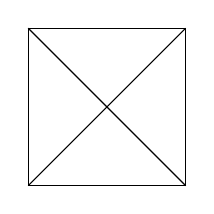
\begin{tikzpicture}
			\draw (0,0) rectangle (2,2); % Draw the square
			\draw (0,0) -- (2,2); % Draw the first diagonal
			\draw (0,2) -- (2,0); % Draw the second diagonal
		\end{tikzpicture}
	\end{center}
	The vertices are indexed by pairs of elements of the Weyl group. The edges are indexed by \red{???}.
	To reason about this one asks the question of which matrices are stabilized when you act on the left and right by $T$.
	The answer is the ones with only one coordinate nonzero. The 1-dimensional orbits are understood similarly.
	There is a submoment polytope for the $\P^1\times \P^1$ orbit:
	\begin{center}
		\begin{tikzpicture}
			\draw (0,0) rectangle (2,2); % Draw the square
		\end{tikzpicture}
	\end{center}
	where you forget the diagonal lines. There was a remark that really the moment polytope for $\bar G$
	should be a tetrahedron but we projected it down to a square. Allen also remarked that permutation matrices are
	correct in this setting, but if we were talking about the whole matrix space instead of $\PGL(2)$ then
	the correct answer is really partial permutation matrices.
\end{example}
\section{Homework}
Finally Allen told us to study the $B\times B$ orbits in $\bar G$. We will think about the $\PGL(2)$ example in the context
of the divided difference operators when we return. We also need to meet with Tara.

\hfill

The question is what should we do for next week? What direction are we moving in? If I understand correctly
we are trying to apply the machinery of the Bott Samelson crank to develop an understanding of
equivariant divided difference operators on the equivariant cohomology of the wonderful compactification.

\hfill

This means that we should probably study the following things:
\begin{enumerate}
	\item Bott Samelson crank and equivariant divided difference operators
	\item $B\times B$ orbits in $\bar G$. One should think of this as analagous to Bruhat decomposition
\end{enumerate}

\section{Wonderful compactification}
Recall the wonderful compactification associated to a reductive adjoint group $G$. Reductive means at all
representations of $G$ decompose as a direct sum of irreducible representations. Adjoint means that the center 
is trivial.

\hfill

Let $\tilde G (\SL(n)$ denote the universal cover of $G (\PGL(n))$ and pick $V$ a representation of $\tilde G$ of 
highest weight $\lambda$. In particular we ask that $\lambda$ is regular, meaning that it lies in 
the interior of the Weyl chamber. The boundary of the Weyl chamber are known as the walls. Note that it is enough
to actually take $V$ to be a reducible representation which contains a copy of such a irreducible representation.

Then there is a map $\tilde G \to \End V \backslash 0$ which descends to a map $G \to \P(\End V)$ because we 
chose $\lambda$ to be regular. The Zariski closure of the image of this map is the wonderful compactification $\bar G$.

\begin{example}[$\PGL(3)$]
\end{example}
    

\end{document}